\section{Tvorba datasetu}
\label{sec:Chapter41}

Dataset byl rozdělen v poměru 70:15:15. Každý kompozit vygenerovaný pro danou sadu byl tvořen snímkem pozadí i zájmového objektu dostupného pouze pro danou sadu. Po vygenerování datasetu byl počet finálních snímků 9009:1929:1939, kde každé vykreslení auta v jednom z 5 možných scén je použito právě jedenkrát pro každý výsledný kompozit. K augmentaci dat byl navržen dvouprůchodový proces, kde první stupeň provedl afinní transformace modelu auta a druhý stupeň vizuální augmentaci kompozitu. Součástí tohoto procesu byla také transformace pozic klíčových bodů a ohraničujících boxů.

V datasetu jsou zahrnuty následující augmentace modelu a kompozitu:
\begin{itemize}
\item \textbf{Afinní transformace modelu} -- otáčení, posun, změna velikosti
\item Náhodná změna jasu, kontrastu, sytosti a tónu
\item Náhodná úprava gamy (světlosti/tmavosti)
\item Vyrovnání histogramu (kontrast)
\item Rozmazání a zaostření
\item Gaussovský šum, ISO šum, JPEG/WebP kompresní chyby
\item Atmosférické efekty -- Mlha, sníh, déšť
\item Optické zkreslení kamery
\end{itemize}


\begin{figure}[ht]
\centering
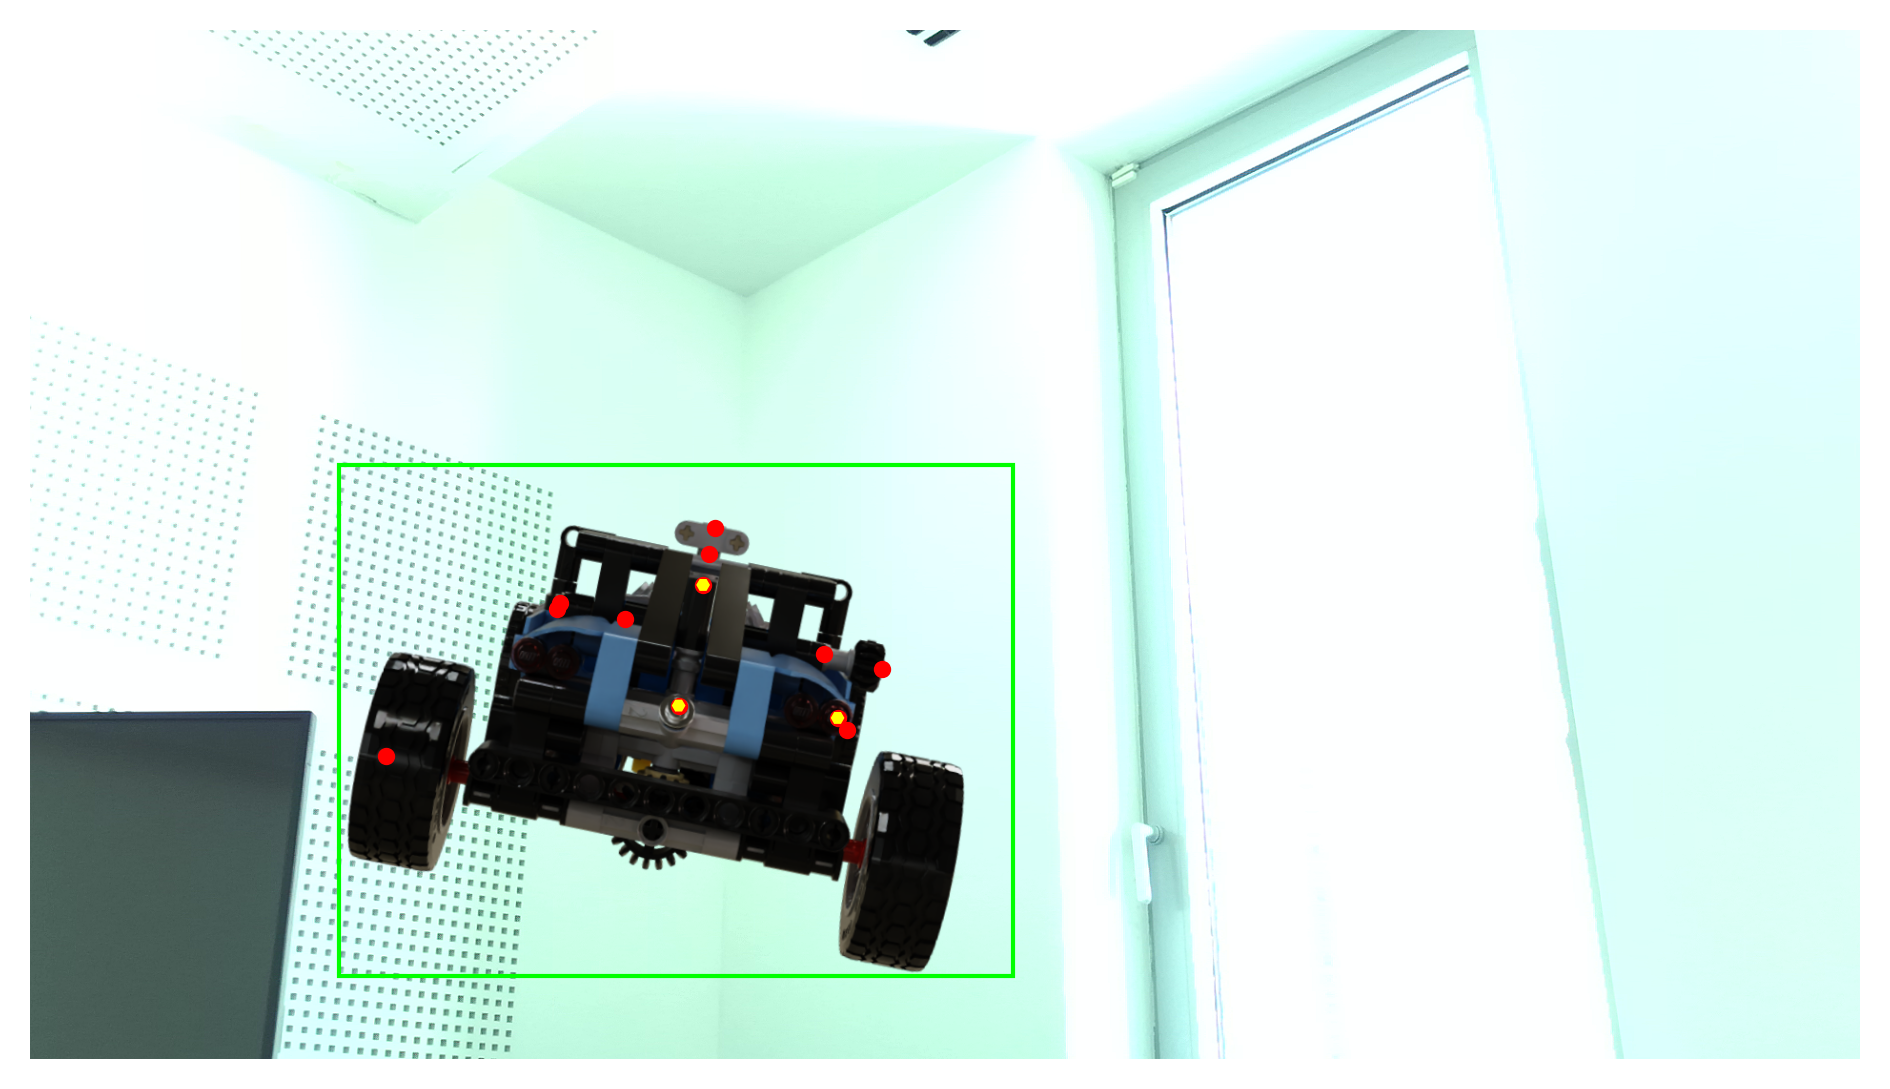
\includegraphics[width=0.5\textwidth,keepaspectratio]{Figures/dataset_ex.png}
\caption[Ukázka transformovaného kompozitu]{Ukázka transformovaného kompozitu, červené body jsou klasifikovány jako neviditelné, zatímco žluté jsou v dostatečně nízkém úhlu pohledu vůči kameře (<75°).}
\label{fig:datasetimg}
\end{figure}